\setchapterimage[6.5cm]{Grid_FullView_Logo}
\setchapterpreamble[u]{\margintoc}
\chapter{Statistical Analysis in IceCube}
\labch{llh}
\begin{fquote}[Ronald Fischer][The Design of Experiments][1935]Every experiment may be said to exist only in order to give the facts a chance of disproving the null hypothesis.
\end{fquote}

As a field, Neutrino Astronomy is still very much in its infancy. While most branches of astronomy are focussed on characterising the properties of astrophysical objects, neutrino astronomy primarily seeks to just identify such objects in the first place. Given the characteristic signal-to-noise of neutrino detectors, determined by their limited resolution and event rate with an enormous atmospheric background, a significant fraction of correlations in data will be due simply to background fluctuations. This statement applies both to clustering within the neutrino data, and to correlations between neutrinos and external data.

Neutrino astronomy is thus predominantly a process of statistical analysis, seeking both to identify correlations and to evaluate whether these are coincidental or physical. As introduced in Chapter \ref{ch:icecube}, we have access to three key observables when performing this analysis with IceCube:

\begin{itemize}
	\item \textbf{Event arrival time}, $t$, with nanosecond precision.
	\item \textbf{Reconstructed direction},  zenith ($\theta$) and azimuth ($\phi$), in local detector coordinates. This quantity has a significant uncertainty, which can also be estimated, providing an additional observable ($\sigma$). The reconstructed direction, in combination with the time, can be uniquely mapped to celestial coordinates Right Ascension ($\alpha$) and Declination ($\delta$).
	\item \textbf{Event energy proxy}, $E_{p}$. It can be converted through \emph{unfolding} to give a probability distribution of true neutrino energies, but this requires certain assumptions about the underlying neutrino spectrum and retains typical uncertainties of factor 10.
\end{itemize}

This chapter outlines the process by which these observables are analysed, and correlations are established. A software designed to perform such analysis,  \flarestack{}, was developed by the author to study correlations in IceCube data \sidecite{flarestack}.

\section{Hypothesis Testing}
Neutrino Astronomy with IceCube uses a \emph{Frequentist} approach to statistical inference, and in particular uses the method of \emph{statistical hypothesis testing} to establish correlations. Statistical hypothesis testing begins with the definition of a particular hypothesis to test, $\mathcal{H_{1}}$, and a null hypothesis, $\mathcal{H_{0}}$, that would be expected in the absence of any correlation. Ultimately, we wish to determine which hypothesis better describes our data. Hypothesis testing adopts the default position that the null hypothesis describes the data, and evaluates whether this description can be disproven. We define a test statistic (TS) to quantify how well data is described, and define a threshold at which we would be confident in reaching a conclusion. If our test statistic exceeds this threshold, we \emph{reject the null hypothesis}. This means we are confident that the null hypothesis does not describes our data. It does not necessarily follow that our signal hypothesis is correct, we can only say that it better describes our data than the null hypothesis. Conversely, if the TS does not exceed the threshold,  we \emph{do not reject the null hypothesis}. In this case, we are not confident that the null hypothesis does not describe our data. This does not mean that the signal hypothesis is wrong, but rather that we cannot be sure the null hypothesis is wrong. 

\begin{margintable}
	\caption[]{Hypothesis Testing}
	\raggedright
	\begin{tabular}{ c|  c c}
		\hline
		& not rejected & rejected \\
		\hline
		$\mathcal{H_{0}}$ true & \cmark & Type I \\
		$\mathcal{H_{0}}$ false &Type II & \cmark\\
		\hline
	\end{tabular}
	\label{tab:hypothesis}
\end{margintable}

As illustrated in Table \ref{tab:hypothesis}, there are two things that can go wrong with a hypothesis test. Type I error, or a false positive, occurs when we reject the null hypothesis although it is true. Type II error, or a false negative, occurs when we do not reject the null hypothesis even though it is false. By construction, every test must balance the risk of Type I and Type II errors, and both cannot be eliminated simultaneously. We typically construct our test by fixing a threshold for acceptable rate of Type I error. This Type I error rate is quantified by a \emph{p-value}, defined as the probability of observing a result under the null hypothesis that is at least as significant as the one found. One common p-value threshold is 0.05, i.e only accepting results with a probability <5\% to arise under the null hypothesis. The p-vaue can also be converted to a \emph{significance}, equal to the number of standard deviations required for a one-sided Gaussian distribution to yield that p-value. A typical threshold for a discovery, common in particle physics, is $5 \sigma$. This corresponds to a p-value of less than $3 \times 10^{-7}$.

While the simplest hypothesis test is a binary case is which one well-defined hypothesis $\mathcal{H_{1}}$ is compared to the null hypothesis, the procedure is often generalised to cover multiple hypotheses, $\mathcal{H_{i}}$, which can be either discrete or continuous. We pick the hypothesis with the smallest p-value, and compare that to our null hypothesis.

\section{Null Hypothesis and Background Modelling}
\label{sec:background}

For neutrino astronomy, the null hypothesis is that \emph{events are distributed according to the background model}. At the stage of defining background models, IceCube-specific physics is added to the pure mathematical basis of hypothesis testing. As outlined in Chapter \ref{ch:event_selection}, IceCube data in the northern hemisphere is dominated by the \emph{atmospheric neutrino background}, while events in the southern hemisphere are dominated by \emph{atmospheric muon bundles}, and in both hemispheres the astrophysical neutrino component is subdominant. This astrophysical neutrino flux likely consists of components from multiple source classes, so there is in principle an additional \emph{astrophysical background} for contributions not included in the signal hypothesis.

It is common in IceCube to take the simplifying assumption that \emph{the data is sufficiently background-dominated to be used as a background model}. The motivation is twofold, it is firstly approximately true, but more importantly the colossal muon rate (\sim3kHz) makes it very difficult to simulate the small fraction of muons which form a signal-like background for the southern hemisphere \sidecite{icecube_detector_17}. In the absence of any adequate simulated model for background in the southern hemisphere, we are forced to instead use a data-based model as a null hypothesis. 

The simplification has a number of drawbacks, primarily that Probability Density Functions (PDFs) derived from data are necessarily coarser because the available statistics are limited. An alternative approach, used for the sample of northern through-going muons tracks in which there is negligible atmospheric muon background, is to use Monte-Carlo based modelling to construct a model for background \sidecite{ic_diffuse_8year}. This ultimately introduces the risk of data-MC disagreement,  with uncertainties introduced for example with by atmospheric and astrophysical flux modelling. However, this is typically offset by the high-resolution PDFs which can be constructed using these much larger sample sizes.

In either case, distributions are then constructed for the background model $\mathcal{B}$. Using our observables , we can construct a composite background model consisting of a spatial, temporal and energy component:

\begin{equation}
\mathcal{B} (t, \theta, \phi, \sigma, E_{p}) =  \mathcal{B}_{\textup{time}} \times  \mathcal{B}_{\textup{space}} \times\mathcal{B}_{E}
\end{equation}

In the following, data-based background PDFs are illustrated for the IceCube all-sky ten year point source dataset (\emph{`ps tracks version v003-p02'}) \sidecite{ic_ps_10_yr}.

\subsection*{Background Time PDF}

The IceCube detector is characterised by extremely high uptime of >99\%, divided into runs separated by small downtime breaks. Even after processing to final-level event selections, samples typically consists of livetime at >90\%, with the remaining time lost to partial detector operation, testing or temporary DOM failure. The arrival time of background events in Icecube is typically \emph{assumed to be uniform during detector uptime}. This is again only approximately true, as evidenced by Figure \ref{fig:background_rate}.  Six peaks corresponding to winters in the northern hemisphere are clearly visible, corresponding to $\pm \sim5\%$ rate variations.

The atmospheric background rates depend on atmospheric densities which are ultimately temperature-dependent, leading to seasonal variations and clearly-visible annual cycles. This variation is itself an area of scientific interest, being exploited to measure climate variations with neutrinos \sidecite{seasonal_neutrinos}. These effects are partially mitigated in data-based models by the standard method of shuffling measured neutrino arrival times rather than drawing them from a PDF. In any case, the arrival time anisotropy is a small one.

Given this, we can approximate the background time PDF as uniform over periods of detector operation, with normalisation:

\begin{equation}
\mathcal{B}_{\textup{time}} \approx \frac{1}{\textup{livetime}}
\end{equation}

\begin{figure}[!ht]
	\centering 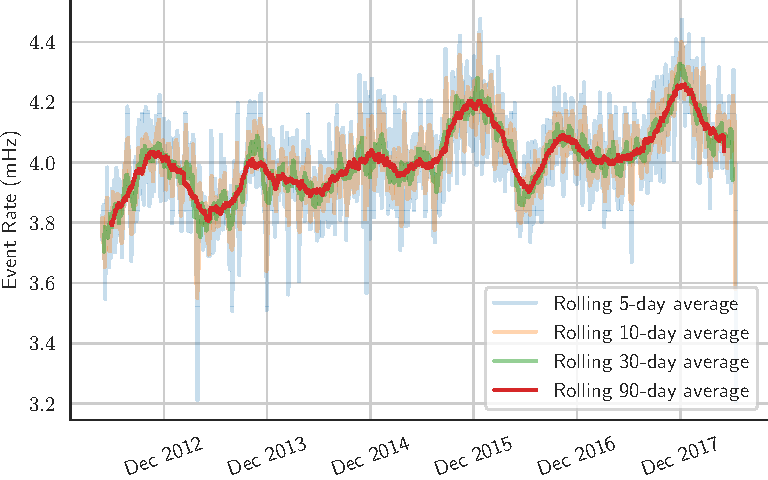
\includegraphics{llh/background_rate}
	\caption{Rolling average of final-level event rate during detector uptime.}
	\label{fig:background_rate}
\end{figure}

\subsection*{Background Spatial PDF}

The spatial distribution of the background can be neatly factorised into two distinct components, namely a zenith and an azimuth component:

\begin{equation}
	\mathcal{B}_{\textup{space}} (\theta, \phi) = \mathcal{B}_{\theta}(\theta) \times \mathcal{B}_{\phi}(\phi, \theta)
	\label{eq:b_space_local}
\end{equation}


\begin{marginfigure}
	\centering 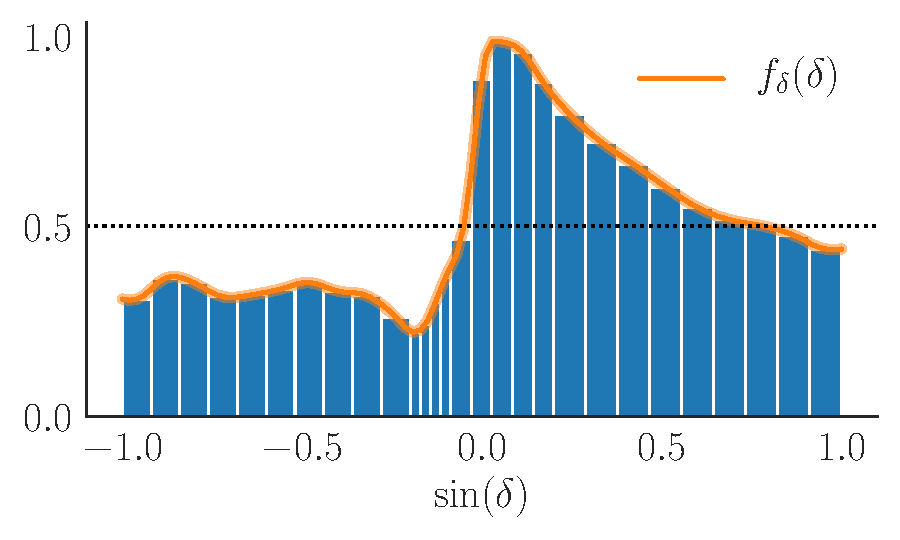
\includegraphics{llh/sindec}
	\caption{Event rate as a function of $\sin(\delta)$.}
	\label{fig:sindec}
\end{marginfigure}

Owing to IceCube's convenient location at the geographic south pole, the zenith-dependent detector response can be uniquely mapped into a declination-dependent one. With a data-driven background model, we can define a PDF $f_{\delta}(\delta)$ based on the declination-dependent event rate, as seen in Figure \ref{fig:sindec}.

\begin{equation}
	\mathcal{B}_{\delta}(\delta) = f_{\delta}(\delta)
	\label{eq:b_theta}
\end{equation}

The additional azimuthal component can be seen in Figure \ref{fig:azimuth}. The detector itself (see Chapter \ref{ch:icecube}) has 6 string axes, and these are clearly visible with elevated event rates. These variations reach up to $\sim40\%$ variations for the southern hemisphere. Additionally, the impact of \emph{ice anistropy} can be seen from an event rate deficit at and below the horizon \sidecite{ic_birefringence_19}, aligned with the axes of maximal charge deficit at $\sim2\pi / 3$ and $5\pi / 3$. 

\begin{marginfigure}
	\centering 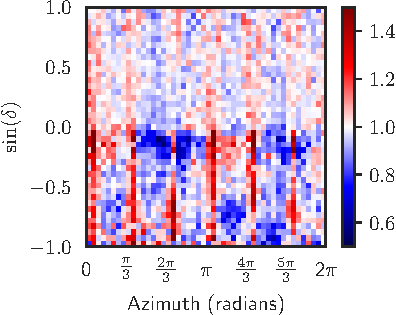
\includegraphics{llh/azimuth}
	\caption{Declination-normalised event rate as a function of azimuth.}
	\label{fig:azimuth}
\end{marginfigure}

However, string axes will all be traced out over the course of each day. Thus, for typical data periods of many years, these azimuthal variations will be averaged out. It is therefore typically assumed that \emph{any variations due to azimuthal asymmetry are negligible}.  An exception must be made for searches targeting clustering over short (sub-day) time periods, where this azimuthal asymmetry may have an impact. Beyond this, as long as the azimuth asymmetry can be neglected, we then find that the distribution in right ascension is uniform:

\begin{equation}
	\mathcal{B} (\alpha) = \frac{1}{2\pi}
	\label{eq:b_alpha}
\end{equation}

By substituting Equations \ref{eq:b_theta} and \ref{eq:b_alpha}, we can then replace Equation \ref{eq:b_space_local} with:

\begin{equation}
	\mathcal{B}_{\textup{space}} (\delta) = \frac{1}{2\pi} \times f(\delta)
	\label{eq:b_space}
\end{equation}

\subsection*{Background Energy PDF}

\begin{marginfigure}
	\centering 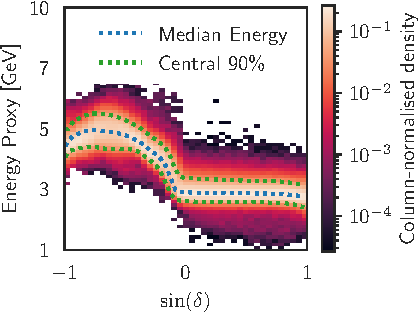
\includegraphics{llh/dec_vs_energy}
	\caption{Background energy proxy distribution, normalised in bins of $\sin(\delta)$.}
	\label{fig:dec_vs_energy}
\end{marginfigure}

Having factorised the declination dependence of events in equation \ref{eq:b_theta}, we can then consider the expected energy proxy distribution for a given spatial position. The normalised energy proxy distribution as a function of $\sin(\delta)$ is given in Figure \ref{fig:dec_vs_energy}, with the median and central 90\% ranges marked by dotted lines. It is clear that in the northern hemisphere, this distribution is essentially flat, reflecting the homogeneity of atmospheric neutrino backgrounds in this regime. However, the median energy proxy swiftly increases into the southern hemisphere, as more aggressive cuts are employed to remove the additional atmospheric muon background. The final turnover at the pole reflects the impact of the IceTop surface detector, which can be used to veto muon bundles from vertically-inclined showers.

\begin{marginfigure}
	\centering 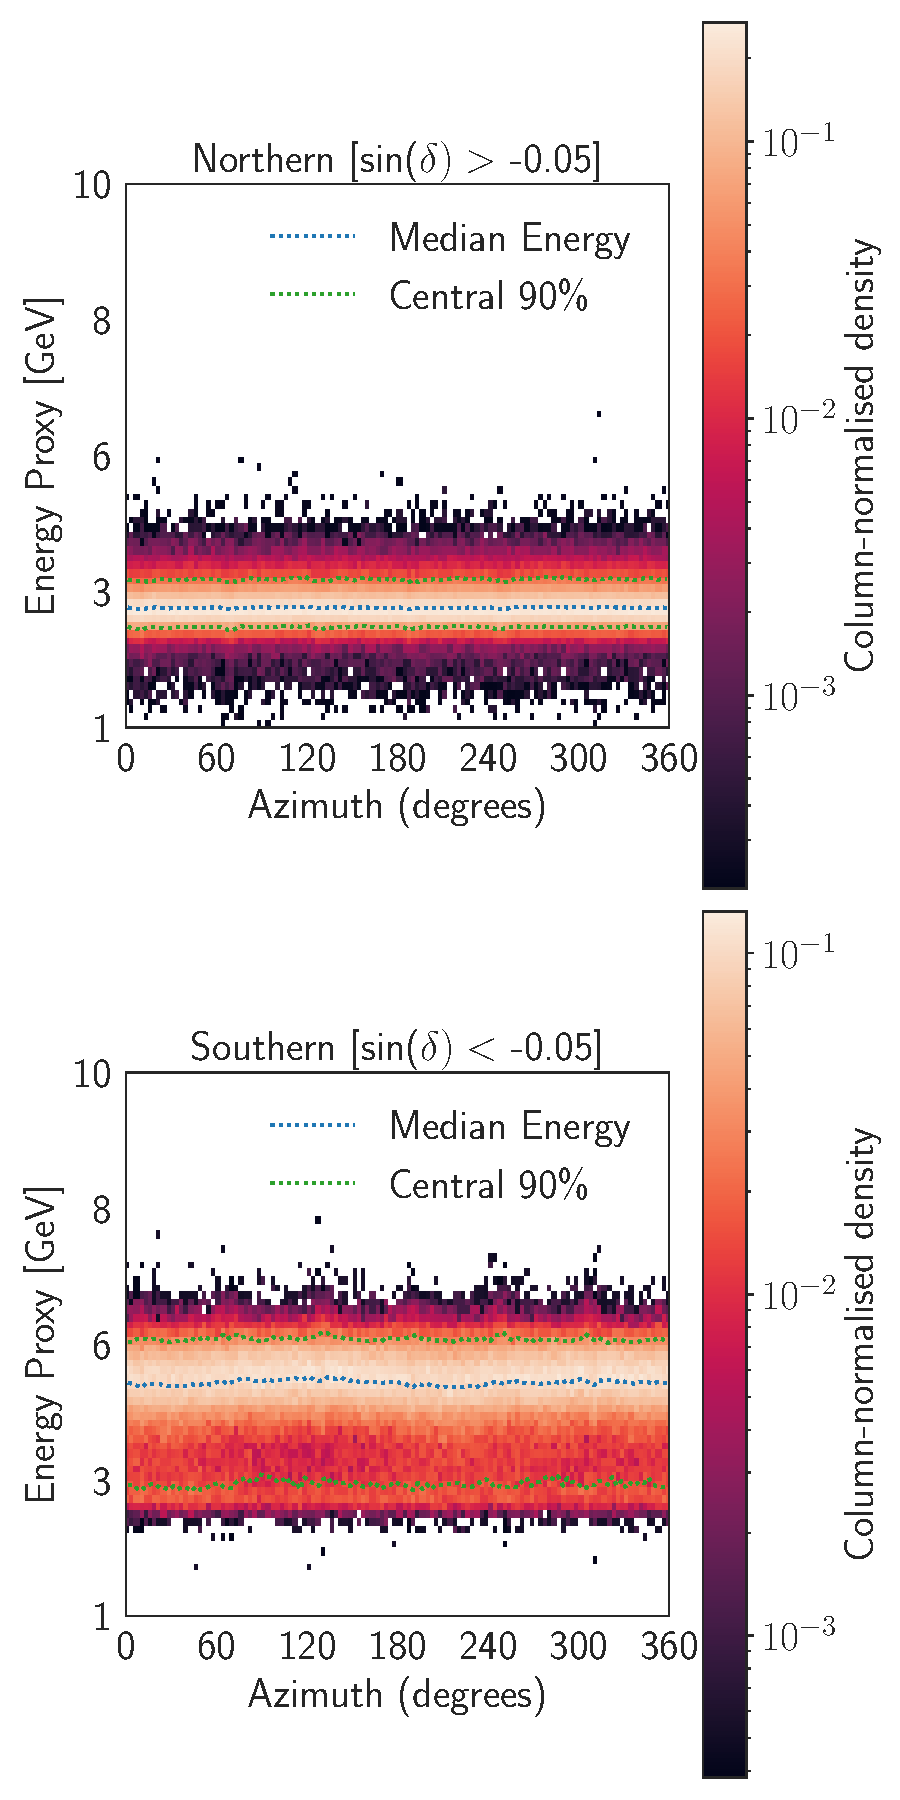
\includegraphics{llh/az_vs_energy}
	\caption{Background energy proxy distribution, normalised in bins of azimuth.}
	\label{fig:az_vs_energy}
\end{marginfigure}

In contrast to the strong declination dependence, Figure \ref{fig:az_vs_energy} shows that there is a no azimuthal dependence for events in the northern hemisphere, and negligible variation in the southern hemisphere. We can thus construct simple two-dimensional background energy PDFs using the distribution shown in Figure \ref{fig:dec_vs_energy}:

\begin{equation}
\mathcal{B}_{\textup{E}} (\delta, E_{\textup{proxy}}) = f_{\textup{E}}(E_{\textup{proxy}}, \delta)
\label{eq:b_energy}
\end{equation}

\section{Signal Hypothesis}
\label{sec:signal}

Signal hypotheses in IceCube are a composite of the background model with a small number of additional signal-like neutrinos ($n_{s}$). It is assumed that \emph{the total number of neutrino events is essentially fixed by background}, so that N = $n_{s} + n_{b}$. In this case, we define our signal hypothesis as the normalised sum of a background PDF $\mathcal{B}$ and signal PDF $\mathcal{S}$:

\begin{equation}
\mathcal{H}= \frac{n_{s}}{N} \mathcal{S} + \frac{N - n_{s}}{N} \mathcal{B} 
\label{eq:sig_hypo_single}
\end{equation}

Much like the background, the signal PDF is a product of energy, temporal and spatial PDFs:

\begin{equation}
\mathcal{S} =  \mathcal{S}_{\textup{time}} \times  \mathcal{S}_{\textup{space}} \times\mathcal{S}_{\textup{E}}
\end{equation}

In IceCube, it is common to test hypotheses in which the the number of signal neutrinos, $n_{s}$, is a free parameter. It is also common to assume that the intrinsic signal energy PDF is an unbroken power law with some spectral index, $E^{-\gamma}$, where the spectral index $\gamma$ is an additional free parameter. 

\subsection*{Signal Time PDF}

In almost all IceCube analyses, the signal time PDF is assumed to be a uniform distribution over a fixed period of livetime. This could be for the entire duration of a dataset, corresponding to a steady neutrino source. This special case is typically referred to as a \emph{time-integrated analysis}, because it cancels out exactly the assumed background time PDF, yielding a likelihood that does not depend on time. This thesis is concerned with \emph{transient} sources, which are only active over fixed periods of time.  Transient source hypotheses require a \emph{time-dependent analysis}, in which the signal is not assumed to be uniform over the full data-taking duration.

The uptime of the detector can be characterised by a boolean detector response function, $f_{\textup{uptime}}(t)$, that is either on (1) or off (0). The signal time PDF is then a product of the underlying source PDF and this detector response PDF. For this thesis, the only relevant transient time PDF was a simple \emph{box model}. This is a uniform signal normalised over the livetime, $\Delta_{T}$, between start time $T_{0}$ and end time $T_{1}$:

\begin{equation}
\Delta_{T} = \int_{T_{0}}^{T_{1}}f_{\textup{uptime}}(t) dt
\end{equation}

\begin{equation}
\mathcal{S}_{\textup{time}} (t)= 
\begin{cases}
	f_{\textup{uptime}}(t) \times \frac{1}{\Delta_{T}} & T_{0} < t < T_{1}\\
	0 & \textup{otherwise}\\
\end{cases}
\end{equation}

\subsection*{Signal Spatial PDF}

The standard spatial signal PDF is typically stated to be \emph{the assumption of a circular Gaussian PSF centered on the position of a source}. For an event at $\vec{x}$ with a localisation uncertainty $\sigma$ and a source at position $\vec{d}$, we then have:

\begin{equation}
r^{2} =  (\vec{x}- \vec{d})^{2}
\end{equation}

\begin{equation}
\mathcal{S}_{\textup{space}} (\vec{x}) = \frac{1}{{2\pi\sigma^{2} }}e^{{{ - r^{2}  } \mathord{\left/ {\vphantom {{ - \left( {x - \mu } \right)^2 } {2\sigma ^2 }}} \right. \kern-\nulldelimiterspace} {2\sigma ^2 }}}
\end{equation}

In reality, even under the limit of a perfect muon track reconstruction, the unmeasurable energy-dependent kinematic angle between the incoming neutrino and outgoing muon will limit the resolution of any search. The signal PSF thus depends on the signal hypothesis, where higher-energy neutrinos are better reconstructed even for fixed $\sigma$. 

Ultimately, the performance of directional reconstructions is verified on MC events, and energy-dependent biases in uncertainty estimates are corrected in a process known as pull corrections (see Chapter \ref{ch:icecube}). So, more precisely, the signal spatial PDF is \emph{assumed to follow the distribution found in baseline MC simulations weighted with an unbroken $E^{-2}$ power law}, and further \emph{it is assumed that this distribution can be approximated by a circular Gaussian PSF with a single per-event energy-corrected uncertainty parameter}. The first assumption clearly requires that the impact of systematic uncertainties on MC simulation is negligible. The validity of these assumptions is discussed further in Chapter N, but it should be noted that neither approximation is completely valid. 

A Gaussian term for the spatial PDF also indirectly \emph{assumes that the Signal PDF does not depend on azimuth}. It is clear in the left panels of Figure \ref{fig:azimuth_mc} that azimuthal asymmetry is increasingly visible for soft spectra in the northern hemisphere, and approximately  resembles the pattern seen in Figure \ref{fig:azimuth}. However, for both the southern sky and a hard E$^{-1}$ spectrum, there is no such asymmetry. As can be clearly seen in Figure \ref{fig:mc_dec_e}, these corresponds to regimes where the signal is dominated by high-energy events. In general, \emph{the effective area at lower energies is azimuth-dependent, while at higher energies it is approximately uniform}. This is because, at lower energies, only tracks which pass close to the DOMs will be detected. In any case, as can be seen in the right-hand panels of Figure \ref{fig:azimuth_mc}, azimuth has very little discriminating power for any spectral index, and can thus be safely neglected for analysis.

\begin{figure}[!ht]
	\centering 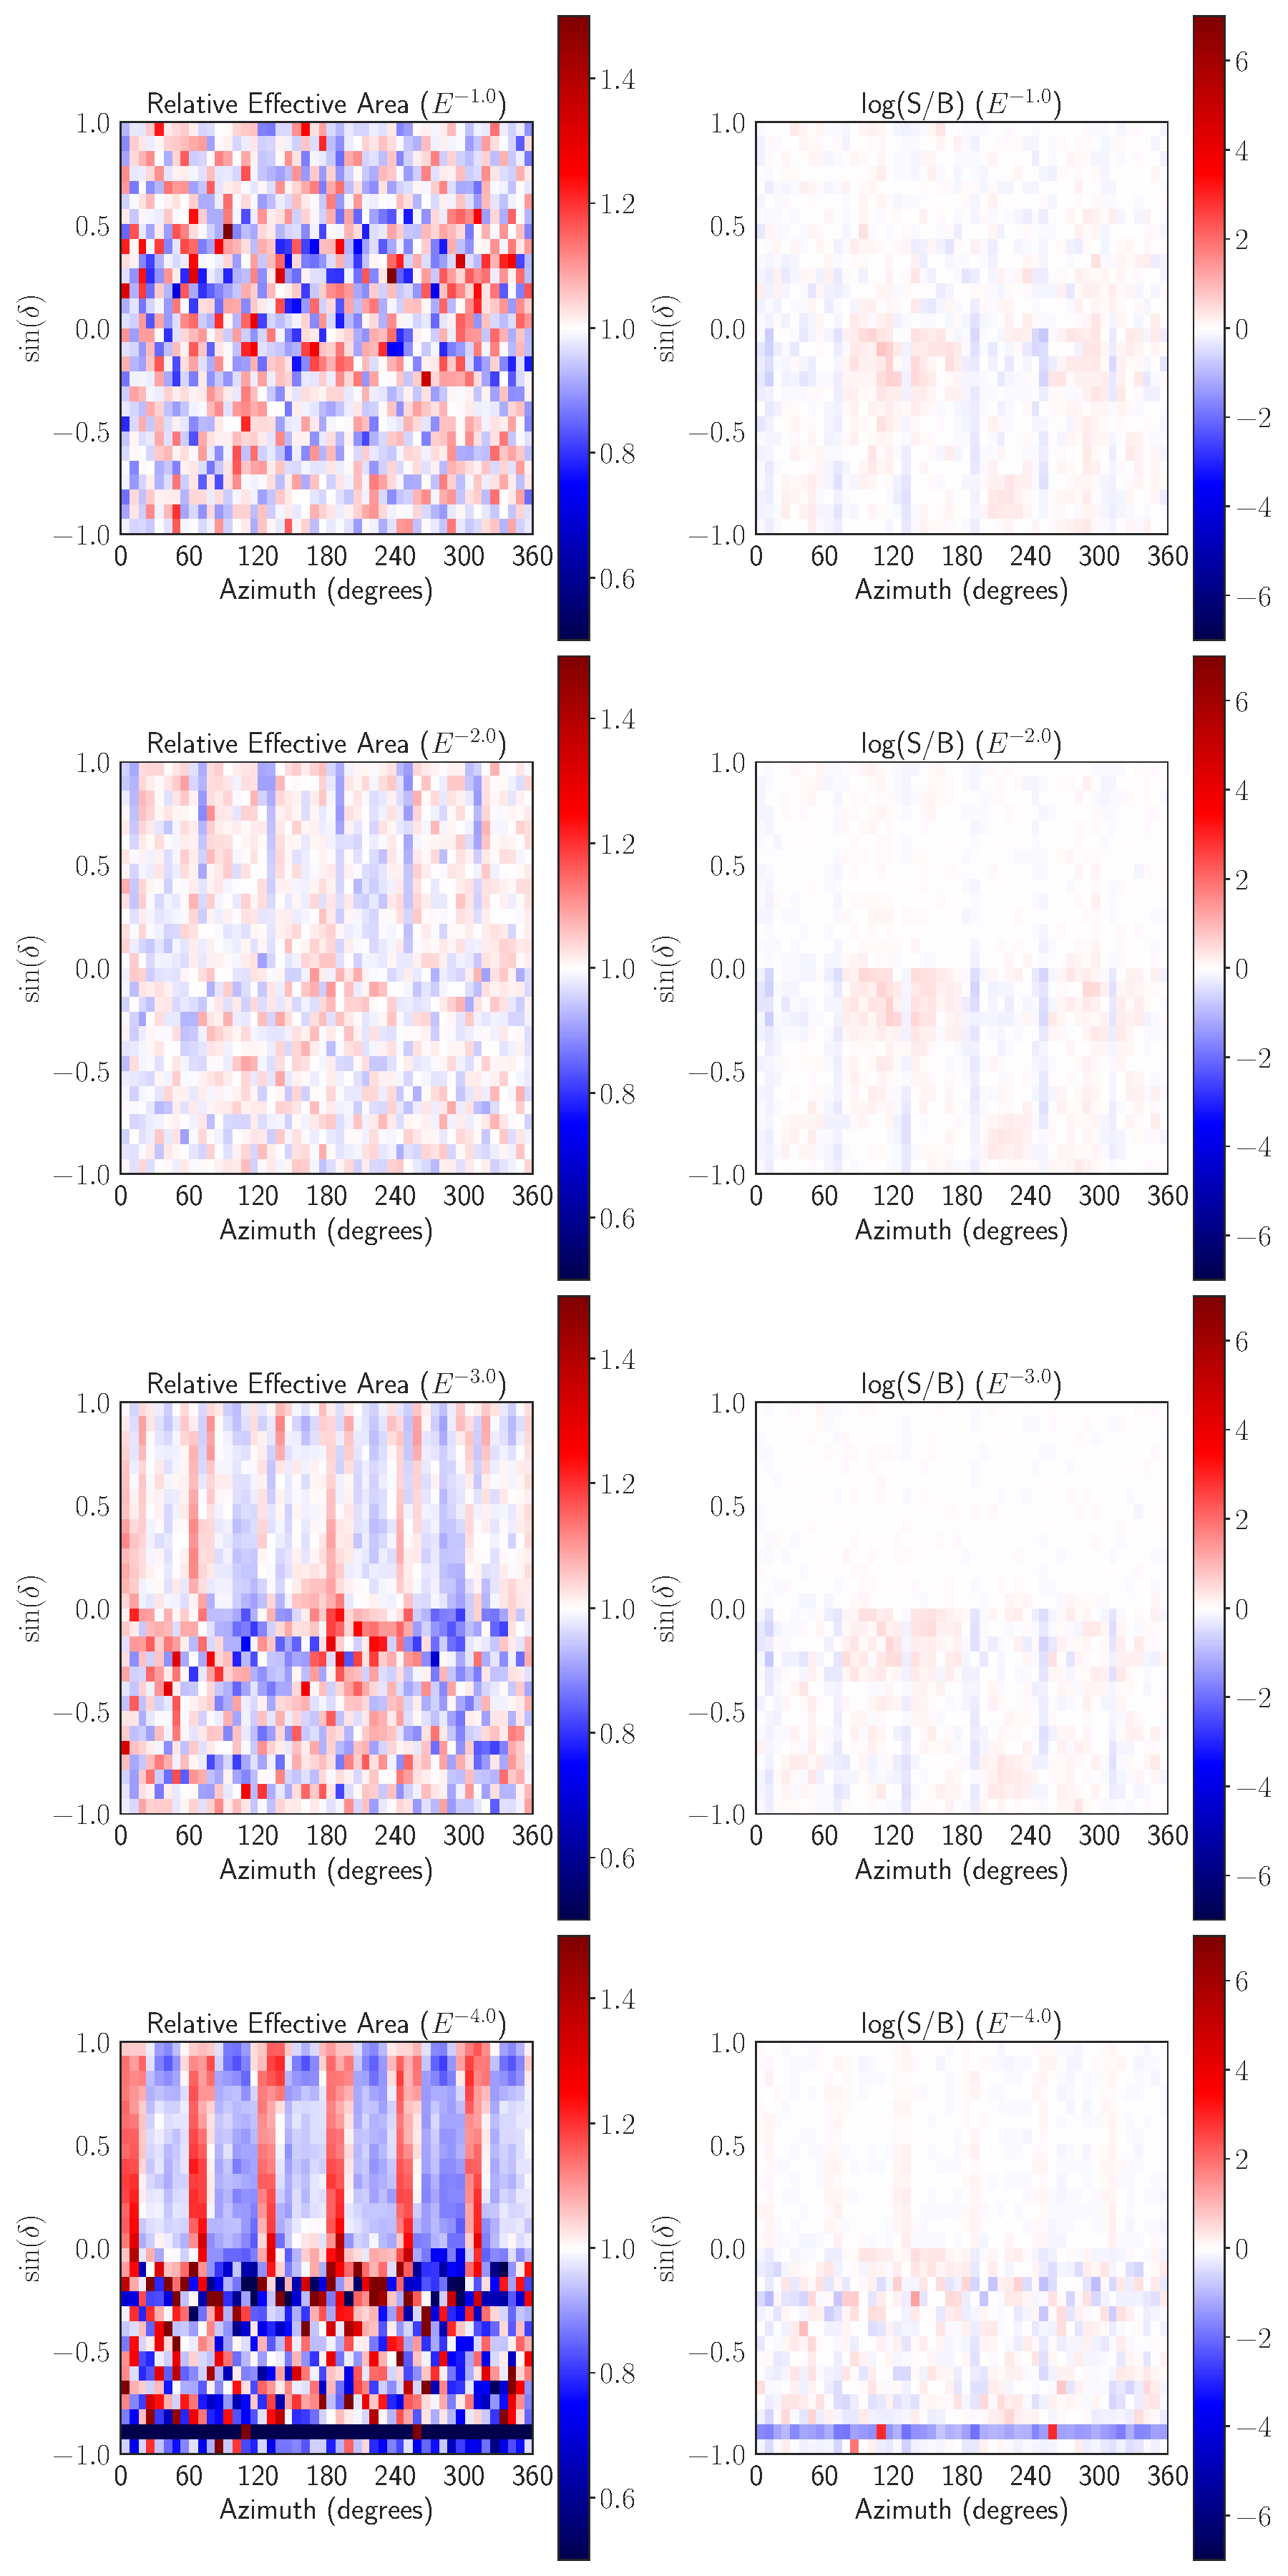
\includegraphics{llh/azimuth_mc}
	\caption{Left: Declination-normalised MC rate as a function of azimuth. Right: Ratio of declination-normalised Signal and Background PDFs.}
	\label{fig:azimuth_mc}
\end{figure}

\subsection*{Signal Energy Proxy PDF}

The energy PDF is most commonly \emph{assumed to be an unbroken power of index $\gamma$ extending over the entire energy range of sensitivity for the IceCube detector}, namely from 100 GeV to 10 PeV. This energy spectrum is then convolved with the detector response function through use of weighted MC simulation, yielding an expected distribution of energy proxy values:

\begin{equation}
\mathcal{S}_{\textup{E}} (\delta, E_{\textup{p}}, \gamma) = f_{\textup{E}}(\delta, E_{\textup{p}}, \gamma)
\label{eq:s_energy}
\end{equation}

An illustration of the expected signal distribution, derived from MC for a range of spectral indices, is illustrated in the left panels of Figure \ref{fig:mc_dec_e}. It is clear that hard spectra result in events with energies substantially above those expected in background, but for softer spectra the distribution narrows and is much more similar to that in Figure \ref{fig:dec_vs_energy}. Much of the discriminating power in IceCube comes from the identification of these high-energy neutrinos, which are unlikely to arise from atmospheric backgrounds but should arise from hard $\sim E^{-2}$ spectra expected for most astrophysical neutrino sources. 

Similar to the spatial PDF, the signal energy proxy PDF \emph{ultimately assumes that the baseline MC accurately describes the expected energy proxy distribution}. This again implicitly assumes that systematic uncertainties have a negligible impact on energy proxy distributions. 

\begin{figure}[!ht]
	\centering 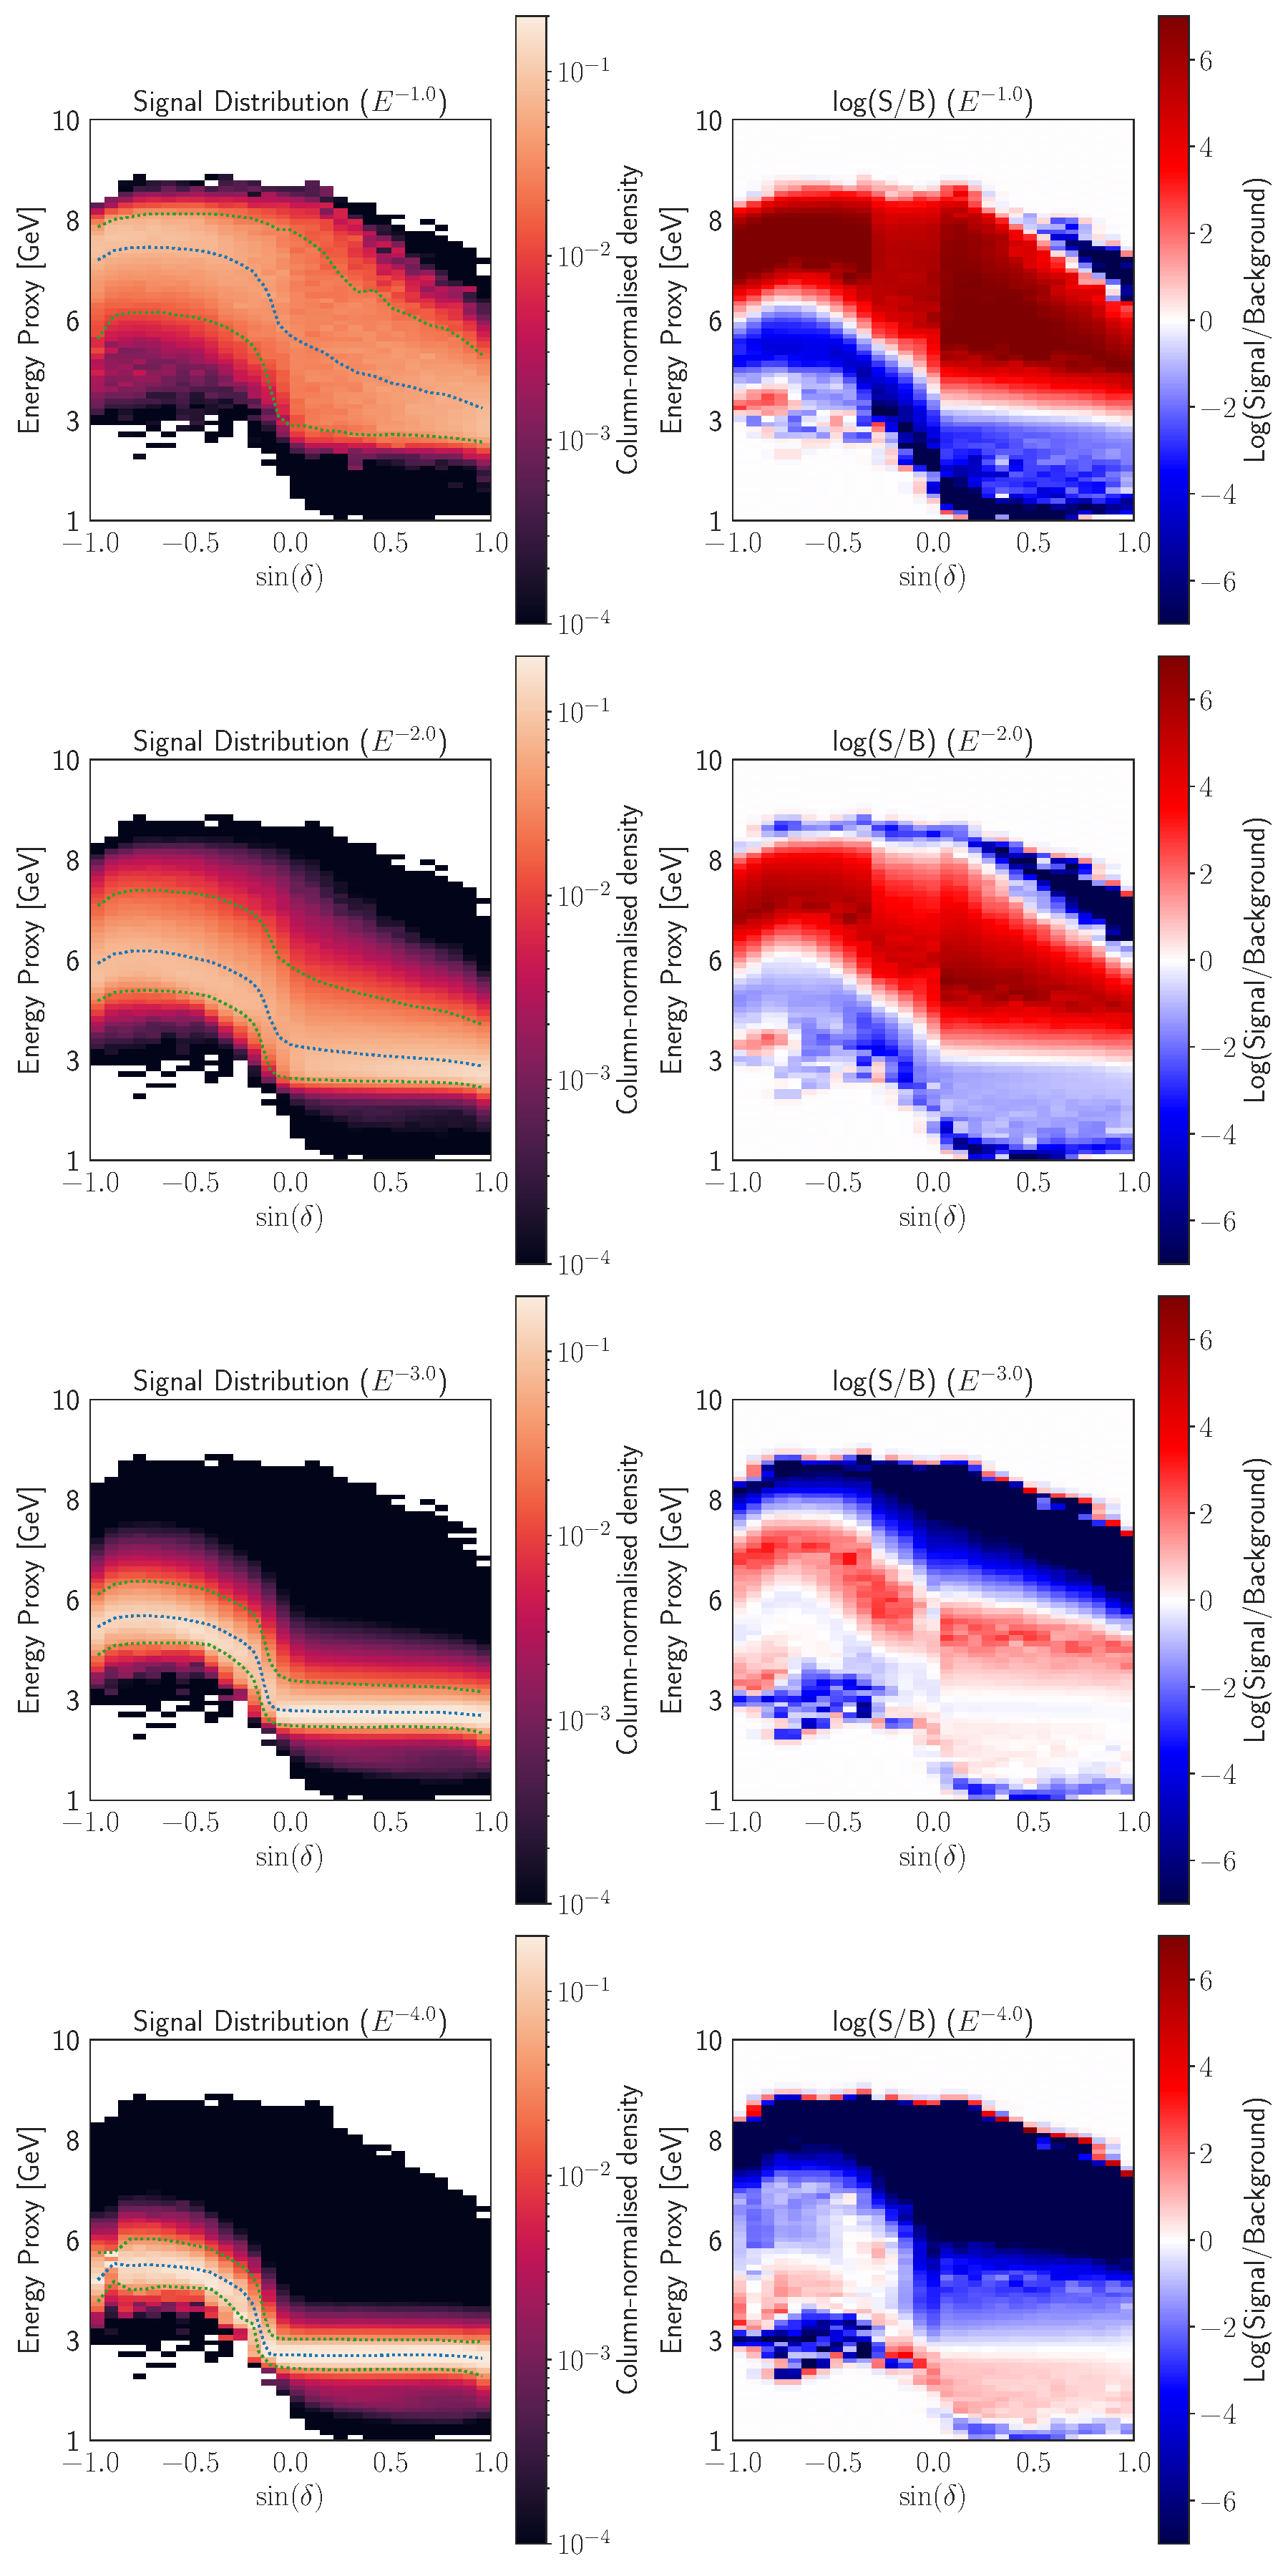
\includegraphics{llh/MC_dec_E}
	\caption{Left: Energy proxy distribution as a function of $\sin(\delta)$, for various signal hypotheses. Right: Ratio of declination-normalised Signal and Background PDFs.}
	\label{fig:mc_dec_e}
\end{figure}

\section{Likelihoods and Wilk's Theorem}

One method of quantifying agreement between a hypothesis and data is to calculate the \emph{likelihood}, $\mathcal{L}$, of observing our data given that hypothesis. Using the PDFs describing how we would expect observables to be distributed for each hypothesis, we can calculate the conditional probability, $\mathcal{L}(x | \mathcal{H})$, of observing our data $x$ given that hypothesis. The likelihood values can be used to construct a test statistic:

\begin{equation}
TS (\mathcal{H_{i}}) = 2 \log \left( \frac{\mathcal{L}(x | \mathcal{H_{i}})}{\mathcal{L}(x | \mathcal{H_{0}})} \right)
\label{eq:ts}
\end{equation}

The primary motivation for using this test statistic definition comes from the \emph{Neyman-Pearson Lemma} \sidecite{1933RSPTA.231..289N}, which states that the likelihood ratio test is the most powerful possible statistical test. 

While this TS definition could also be used for a likelihood that is evaluated for discrete regions of parameter space (a \emph{Binned likelihood analysis}), it has long been customary in IceCube to instead evaulate the likelihood in a continuous event-wise fashion (an \emph{Unbinned likelihood analysis}) \sidecite{braun_ps_methods}. A likelihood is constructed, and evaluated for each jth individual event, with the overall likelihood given by the product of these N independent events:

\begin{equation}
	\mathcal{L} = \prod_{i}^{N} \mathcal{L}_{i}
\end{equation}

Ultimately this yields the standard \emph{Point Source Likelihood}:

\begin{equation}
	\mathcal{L}(n_{s}, \gamma) = \prod_{i}^{N} \left(\frac{n_{s}}{N} \mathcal{S}(\theta_{i}, \gamma) + \frac{N - n_{s}}{N} \mathcal{B}(\theta_{i})  \right)
\label{eq:ps_llh}
\end{equation}

We are thus testing a continuum of hypotheses parameterised by $n_{s}$ and $\gamma$, where both $\mathcal{S}$ and $\mathcal{B}$ depend on the event-specific observables $\theta_{j}$. We typically construct the negative log likelihood ($- \log\mathcal{L}$), and then derive best-fit parameters $\hat{n}_{s}$ and  $\hat{\gamma}$ by a process of maximum likelihood estimation. We take the combination of parameters which maximises the likelihood, and use this as our final TS value. 

\section{Pseudo-trials, P-values and trial corrections}
\label{sec:pvalues}

Given a particular TS value, we must then calculate a p-value to quantify whether or not the null hypothesis can be rejected. The most simplistic method is to perform simulated \emph{pseudo-experiments} based on the null hypothesis, to quantify how often a given outcome occurs. This method critically relies on the assumption that \emph{pseudo-experiments can be accurately simulated, and thus represent the expected distribution}. 

Much like for Section \ref{sec:background}, the null distribution can be simulated using either a data-based or MC-based model. In general, for any point source analysis, data-based methods perform well because the datasets are indeed background-dominated. Furthermore, the data can be easily randomised through use of \emph{data-scrambling}, in which the detector symmetry is exploited by randomly assigning new values of right ascension to events. Furthermore, relying on the assumption that \emph{the dataset is background-dominated at all relevant timescales}, the temporal variations of the background shown in Figure \ref{fig:background_rate} can easily be accounted for by randomly reassigning the arrival time of events to other events. These methods work principally because a point source analysis is concerned with only a tiny fraction of the data, in a narrow right ascension/declination range, and thus the broader population distribution is almost completely independent of any signal hypothesis. Alternatively using MC-based models ensures there is absolutely no contamination of the background distribution with signal, but comes at the cost of introducing a dependence on the data-MC agreement for any subsequent conclusions.

An alternative method of calculating a p-value is to exploit \emph{Wilk's Theorum} \sidecite{Wilks:1938dza}. Wilk's Theorum states that the log likelihood ratio for an ensemble of datasets will be distributed according to a $\chi^{2}$ distribution, with degrees of freedom equal to the number of independent parameters. Thus, for a hypothesis depending on a known number of independent parameters, we can analytically convert any TS value to a \emph{p-value}. There are, however, caveats to Wilk's Theorum. The full formulation only applies in the limit of large samples, and in the absence of bounds on fit parameters. In IceCube this condition is usually satisfied, but there are exceptions particularly for searches on short-timescales relevant for GRB or FRB searches, where the data transitions from a background-dominated regime to a background-free one.

For most cases, including all analysis for this thesis, a hybrid approach is used. A large number of pseudotrials are generated, providing an ensemble of TS values. A $\chi^{2}$ distribution is then fit to this dataset, with the degrees of freedom and normalisation being free parameters. This fitted distribution can then be used to extrapolate from the experimental distribution (typically several hundred thousand) to even smaller p-values, such as for the 5$\sigma$ TS value which would otherwise require several million trials.

\begin{marginfigure}
	\centering 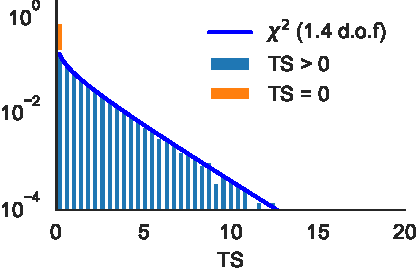
\includegraphics{llh/bkg_ts}
	\caption{Background TS distribution for the standard Point Source Likelihood (Equation \ref{eq:ps_llh}).}
	\label{fig:bkg_ts}
\end{marginfigure}

\begin{marginfigure}
	\centering 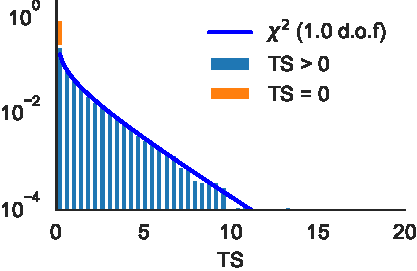
\includegraphics{llh/bkg_spatial_ts}
	\caption{Background TS distribution for a Point Source Likelihood without an energy term.}
	\label{fig:bkg_spatial_ts}
\end{marginfigure}

An example distribution, for a source at the horizon, is illustrated in Figure \ref{fig:bkg_ts}. It is well-fit by the $\chi^{2}$ distribution, with $\sim1.4$ degrees of freedom. Though this may appear to be unphysical, it illustrates the fact that the likelihood outlined in Equation \ref{eq:ps_llh} does not have two independent fit parameters. Rather, given that PS analyses search primarily for an excess of high-energy neutrinos, $n_{s}$ and $\gamma$ are in fact degenerate to a large degree. From the perspective of a likelihood analysis, a single high-energy neutrino on top of an abundant low-energy background does not appear very different to a single high-energy neutrino with a handful of lower-energy neutrinos against an abundant low-energy background. As can be seen in Figure \ref{fig:bkg_spatial_ts}, for a Point Source Likelihood without energy terms, the TS distribution is well fit by a $\chi^{2}$ distribution with exactly 1 degree of freedom, as expected for a likelihood that depends only on $n_{s}$.

For a single hypothesis, the procedure would then be complete. However, it is common that multiple hypotheses are tested at once, for example in this thesis with multiple catalogues (see Chapter \ref{ch:results}). Given that each independent test has a probability to randomly produce an overfluctuation, smaller p-values become increasingly likely as more tests are added. To counteract the multiple hypothesis problem, known as the \emph{look-elsewhere effect}, a correction must be introduced, known as a \emph{trial factor}. The trial factor quantifies the number of independent tests that have been performed, and thus quantifies how likely it is to find a small p-value. If the smallest pre-trial p-value is $p_{\textup{pre-trial}} $, then for N independent trials we find:

\begin{equation}
p_{\textup{post-trial}} = 1 - \left( 1 - p_{\textup{pre-trial}} \right)^{N}
\label{eq:trial_correction}
\end{equation}

Defining what constitutes an independent trial can be difficult. It is a common misconception that the trial factor is particularly important for cases when two hypotheses are similar. In the limit that two hypotheses are so similar as to be essentially identical, there would be no need for a trial correction at all, since the test statistic for each would be identical. The trial factor should correct the degree to which hypotheses are capable of giving multiple independent TS values. Distinct catalogues which do not share sources are completely independent trials, and thus N is simply the number of source lists tested. For correlated tests, such as overlapping catalogues or identical catalogues with different intrinsic source weighting, the trial factor will always be smaller than the number of tests but there is no analytic solution to the exact factor. Instead, it can in principle be derived experimentally, by performing all tests on each pseudo-trial, and considering the distribution of smallest p-values. In this thesis, the conservative approach is employed instead, by counting tests and assuming they are independent.

\section{Sensitivities, Discovery Potentials and Upper Limits}
\label{sec:sens_uls}

When developing and performing statistical analysis, we often wish to quantify how powerful a particular test is. As an extension of the background pseudo-experiments outlined in Section \ref{sec:pvalues}, we can also perform pseudo-experiments with our signal hypothesis. This is done through the process of \emph{signal injection}, whereby a pseudo-dataset is constructed using a combination of the background model and a signal model. The resulting TS distribution, and all conclusions derived from it, again introduce an assumption \emph{that the baseline MC can be used to represent signal}. 

With a signal TS distribution, we can characterise the power of our test by assessing the degree to which the signal TS distribution differs from the background one. For a given p-value threshold, as defined by the background model, we can calculate how frequently a given signal hypothesis would lead to a rejection of the null hypothesis. This yields the Type II error rate for any test.

The principle can be extended to cover multiple hypotheses. In the case of neutrino astronomy, a signal hypothesis can be defined for any number of signal neutrinos, $n_{\textup{inj}}$, that are injected. Since the detection of neutrinos is a random process, the number of signal neutrinos can be simulated with a poisson process of mean $n_{\textup{exp}}$. We can thus parameterise a continuous set of signal hypotheses as a function of $n_{\textup{exp}}$, under the assumption of a given spectral model. 

\begin{marginfigure}
	\centering 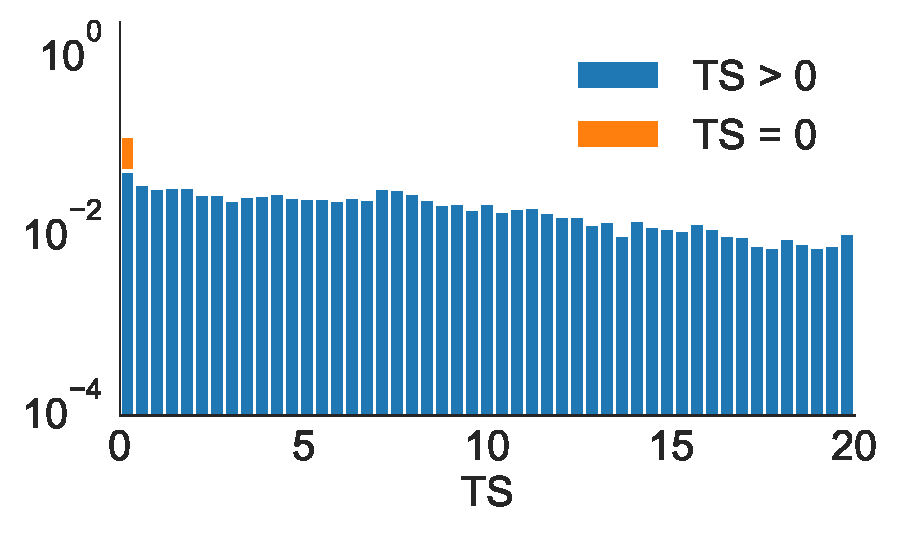
\includegraphics{llh/sig_ts}
	\caption{Signal TS distribution for the standard Point Source Likelihood (Equation \ref{eq:ps_llh}), with $\approx$ 3 injected neutrinos.}
	\label{fig:signal_ts}
\end{marginfigure}

\begin{marginfigure}
	\centering 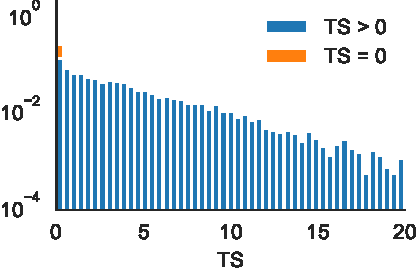
\includegraphics{llh/sig_spatial_ts}
	\caption{Signal TS distribution for the Point Source Likelihood without an energy term, with $\approx$ 3 injected neutrinos.}
	\label{fig:signal_spatial_ts}
\end{marginfigure}

An example signal TS distribution can be seen in Figure \ref{fig:signal_ts}, which covers the same time-integrated horizon source shown in Figure \ref{fig:bkg_ts} with the addition of $\approx$ 3 injected signal neutrinos. The signal TS distribution is notably shifted to higher TS values, with only 6\% of trials yielding a TS=0. The same trend is seen for Figure \ref{fig:signal_spatial_ts}, with the same number of injected signal neutrinos using a spatial-only likelihood.

It is often useful to quantify the rate of both Type  I and Type II errors associated with different regions of parameter space, especially those which rely on $n_{\textup{exp}}$. One example is the \emph{sensitivity} of a test, defined as the value of $n_{\textup{exp}}$ for which 90\% of the signal trials will yield a TS value greater than the background median. Here the Type I error rate is 50\%, and the Type II error rate is 10\%. 

Another common metric is the \emph{median 5$\sigma$ discovery potential}. This is the value of $n_{\textup{exp}}$ for which 50\% of the signal trials will yield a p-value exceeding the 5$\sigma$ threshold. In this case, the Type I error rate is $\approx 3 \times 10^{-7}$, while the Type II error rate is 50\%. The 5$\sigma$ discovery potential illustrates the region of signal parameter space for which a discovery could be expected. 

\begin{marginfigure}
	\centering 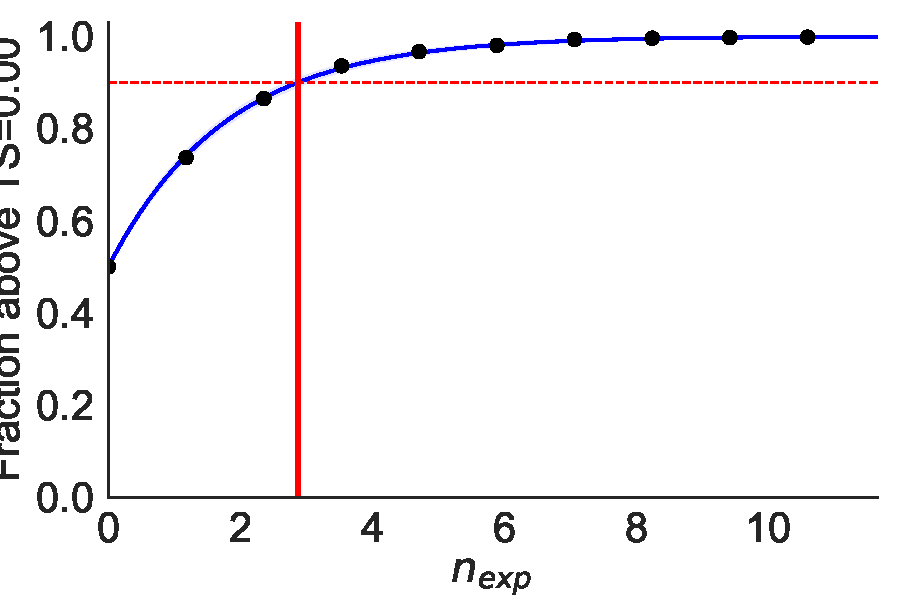
\includegraphics{llh/bkg_ts_sensitivity}
	\caption{Sensitivity for the standard Point Source Likelihood (Equation \ref{eq:ps_llh}),  using the background TS distribution from Figure \ref{fig:bkg_ts}.}
	\label{fig:sens}
\end{marginfigure}

\begin{marginfigure}
	\centering 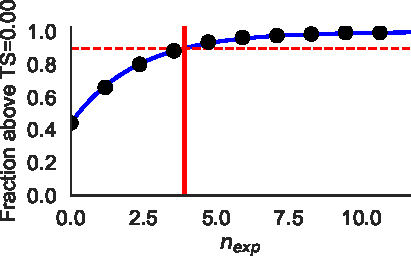
\includegraphics{llh/bkg_spatial_ts_sensitivity}
	\caption{Sensitivity for the Point Source Likelihood without an energy term, using the background TS distribution from Figure \ref{fig:bkg_spatial_ts}.}
	\label{fig:sens_spatial}
\end{marginfigure}

An example of the sensitivity is shown in Figure \ref{fig:sens}, using the background median threshold (TS=0.0)  from the distribution in Figure \ref{fig:bkg_ts}. For comparison, the spatial-only sensitivity is shown in Figure \ref{fig:sens_spatial}, relative to the corresponding background median distribution (TS=0.0) in Figure \ref{fig:bkg_spatial_ts}. While the standard Point Source Likelihood (Equation \ref{eq:ps_llh}) has a sensitivity of $\approx$ 3 signal neutrinos, the spatial-only likelihood has a sensitivity of $\approx$ 4 signal neutrinos. The latter method thus requires $\approx$ 33\% more signal to produce a `likely detection', illustrating the enhanced power of the energy-dependent Point Source Likelihood as a statistical test. The discrepancy is even more extreme for discovery potential, with the standard method requiring $\approx$ 10 neutrinos (Figure \ref{fig:disc}) whereas the spatial-only method requires $\approx$ 18 neutrinos (using the extrapolation in Figure \ref{fig:disc_spatial}). 

\begin{marginfigure}
	\centering 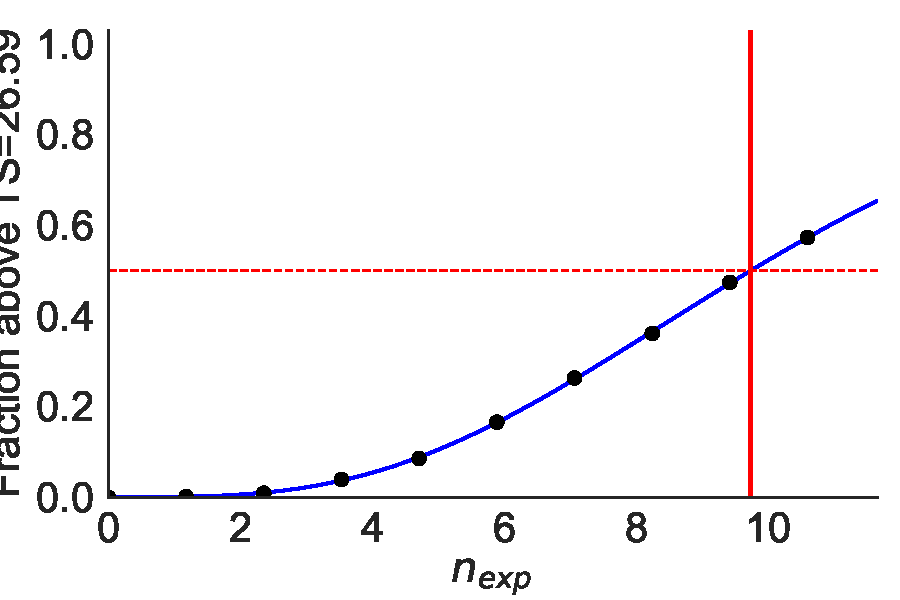
\includegraphics{llh/bkg_ts_disc}
	\caption{5$\sigma$ Discovery Potential for the standard Point Source Likelihood (Equation \ref{eq:ps_llh}), using background TS distribution from Figure \ref{fig:bkg_ts}.}
	\label{fig:disc}
\end{marginfigure}

\begin{marginfigure}
	\centering 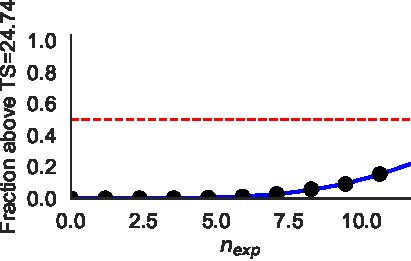
\includegraphics{llh/bkg_spatial_ts_disc}
	\caption{5$\sigma$ Discovery Potential for the Point Source Likelihood without an energy term, using background TS distribution from Figure \ref{fig:bkg_spatial_ts}.}
	\label{fig:disc_spatial}
\end{marginfigure}

These metrics allow us quantify the performance of a test without requiring knowledge of the actual outcome of the test on real data. In this way, an analysis can be designed that is \emph{blind}, and thus free from human bias. We optimise our analysis in terms of achieving the best possible sensitivity or discovery potential, and only then do we perform the test on real data. Applying this principle to the two cases outlined above, it clear that we should use the Point Source Likelihood with an energy term, and this conclusion has been reached without knowledge of the ultimate outcome of either test on the real dataset. 

Once the analysis has been \emph{unblinded}, we can also recycle these pseudo-experiments to set an upper limit. Following exactly the same procedure as for sensitivity, we can derive an upper limit at some confidence level, typically 90\%, using the observed TS value and our pseudo-experiments with added signal. Our upper limit is defined as the signal expectation for which 90\% of the pseudo-experiments would yield a TS greater than or equal to the value observed. By construction, for a median experimental result of the background hypothesis, the upper limit derived at 90\% confidence level is exactly equal to the sensitivity. Conventionally, in IceCube, for results which yield an underfluctuation relative to background expectations (a TS value less than the median), the sensitivity is quoted as an upper limit.

Both sensitivity and discovery potential can be used to characterise and compare the relative power of statistics tests, in terms of signal events. However, through use of the effective area,  $A_{\textup{eff}} (\delta)$, we can convert these values of $n_{\textup{exp}}$ into corresponding values of muon neutrino flux normalisation.

Under the assumption that \emph{the effective area, as derived with baseline MC, is an accurate description of the detector},  we then find for a flux of normalisation $\phi_{0}$:

\begin{equation}
n_{\textup{exp}} (\gamma) = \phi_{0} \int \mathcal{S}_{\textup{time}}(t) dt \int A_{\textup{eff}}(\delta, E_{\nu}) \times E_{\nu}^{-\gamma} dE_{\nu}
\label{eq:n_exp}
\end{equation}

The effective area as a function of declination, $A_{\textup{eff}} (\delta)$, is shown in Figure \ref{fig:effective_area}. The effective area is highest at the horizon (green lines), where it increases with neutrino energy. However, for more northern declination (yellow to red lines), the increasing impact of earth absorption suppresses neutrino detection at energies greater than 100 TeV. For the southern hemisphere, increasingly aggressive cuts to reject atmospheric muons mean that the effective area is also lower overall (blue lines), though as with the horizon there is no earth absorption of neutrinos.

\begin{figure}[!ht]
	\centering 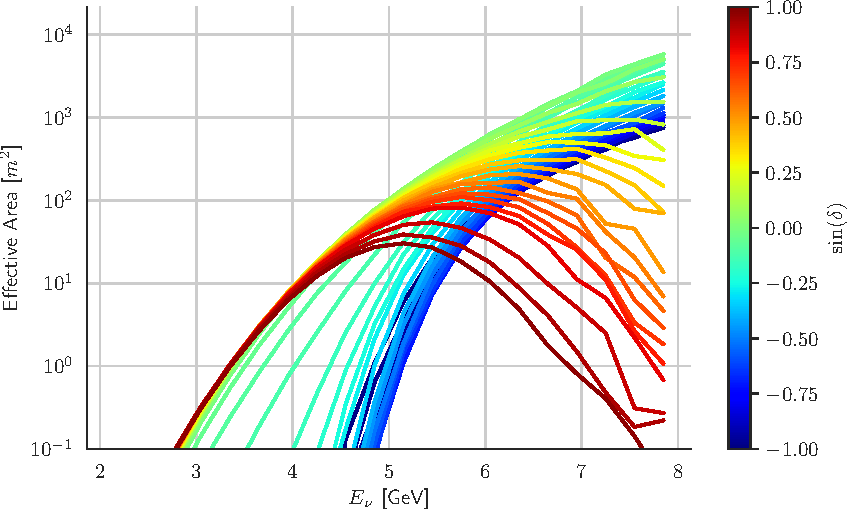
\includegraphics{llh/effective_area}
	\caption{Effective area as a function of neutrino energy and declination.}
	\label{fig:effective_area}
\end{figure}

With Equation \ref{eq:n_exp}, we can then characterise the properties of astrophysical neutrino sources for which we could expect a discovery, and conversely we can constrain these properties for a null result. This is illustrated in Figure \ref{fig:10yr_ps}, illustrating the sensitivity and 5$\sigma$ discovery potential for a point source at various declinations. The values are derived using the full Point Source Likelihood introduced in Equation \ref{eq:ps_llh}, including an energy term. As expected from Figure \ref{fig:effective_area}, the detector is most sensitive at the horizon but gradually deteriorates at more northern declinations due to increasing Earth absorption. Below the horizon, the sensitivity rapidly deteriorates due to the higher muon background.

\begin{figure}[!ht]
	\centering 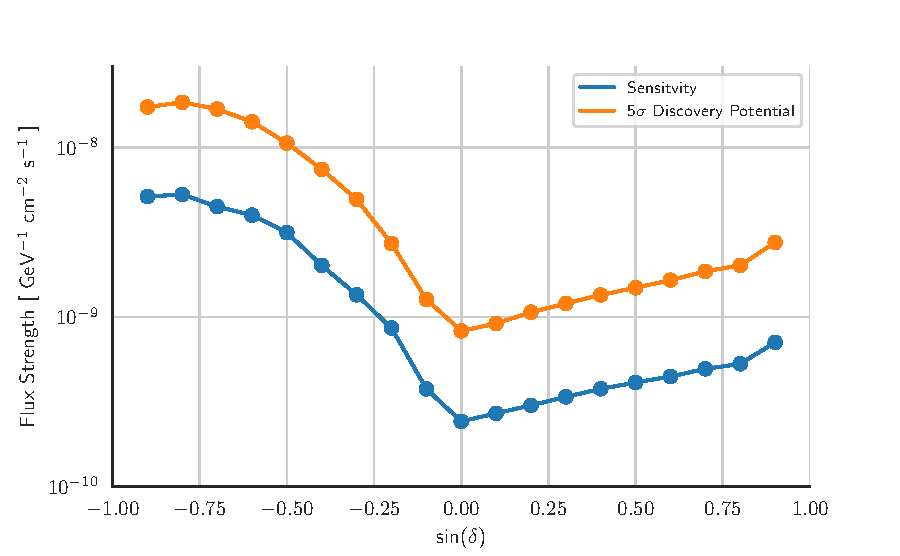
\includegraphics{llh/10_yr_PS}
	\caption{Sensitivity and Discovery potential as a function of declination for an E$^{-2}$ spectrum.}
	\label{fig:10yr_ps}
\end{figure}

\section{Stacking Multiple Sources}

The simple source hypothesis outlined in Equation \ref{eq:sig_hypo_single} describes a single source, but can easily be expanded to include an ensemble of sources, known as a \emph{Stacking Analysis}. For a multi-source hypothesis, the relative contribution of each source must be accounted for.

In most cases, it is \emph{assumed that all sources share the same intrinsic neutrino spectrum}. A further assumption must be made on the fraction of catalogue flux, f$_{k}$, that each kth source will contribute. One common assumption is \emph{equal weights}, so that each of M sources contributes equally:

\begin{equation}
f_{k} = \frac{1}{M}
\label{eq:equal_weighting}
\end{equation}

Alternatively, another common assumption is \emph{standard candles}, where the intrinsic luminosity of each source is equal. For each kth source at lumiosity distance D$_{L,k}$

 \begin{equation}
 f_{k} = \frac{1/D_{L,k}^{2}}{\sum^{M}_{k=1}(1/D_{L,k}^{2})}
 \end{equation}

In any case, we can then calculate the expected number of signal neutrinos, n$_{k}$, for each source:

\begin{equation}
\phi_{k} = \phi_{0} \times f_{k}
\end{equation}

\begin{equation}
n_{k} (\gamma) = \phi_{0} f_{k} \int \mathcal{S}_{\textup{time, k}}(t) dt \int A_{eff}(\delta_{k}, E_{\nu}) \times E_{\nu}^{-\gamma} dE_{\nu}
\label{eq:n_k}
\end{equation}

Using Equation \ref{eq:n_k}, we can then define the fractional source weight, $w_{k}$, of each kth source:

\begin{equation}
w_{k}(\gamma)  = \frac{n_{k}(\gamma) }{\sum^{M}_{k=1} n_{k}(\gamma) } = \frac{f_{k} \int \mathcal{S}_{\textup{time, k}}(t) dt \int A_{eff}(\delta_{k}, E_{\nu}) \times E_{\nu}^{-\gamma} dE_{\nu}}{\sum^{M}_{k=1} \left( f_{k} \int \mathcal{S}_{\textup{time, k}}(t) dt \int A_{eff}(\delta_{k}, E_{\nu}) \times E_{\nu}^{-\gamma} dE_{\nu} \right)}
\end{equation}

Unlike for Equation \ref{eq:n_k}, $w_{k}$ does not ultimately depend on the flux normalisation $\phi_{0}$. For fixed spectral index, the relative contribution of different sources is independent of the number of neutrinos. Using these source weights, we can then define our normalised Signal model:

\begin{equation}
\mathcal{S}(\gamma) = \sum^{M}_{k=1} \left( w_{k}(\gamma)  \times \mathcal{S}_{k}(\gamma)  \right)
\label{eq:S_stacked}
\end{equation}

Substituting this into Equation \ref{eq:ps_llh}, we arrive at our stacked PS likelihood. Conveniently, $\mathcal{S}_{\textup{E}}(\gamma)$ does not vary by source, so can be factorised out of the sum. For steady neutrino sources, $\mathcal{S}_{\textup{time}}$ can also be factorised out, leaving only a sum over $\mathcal{S}_{\textup{space, k}}$.

\section{Combining seasons}

We can generalise the procedure even further, to account for multiple IceCube seasons. As outlined in Chapter \ref{ch:icecube}, the IceCube detector was constructed in phases, with multiple partial detector configurations each operating for roughly one year. It is conventional, as for \emph{ps tracks v003}, to include data from IC40, IC59, IC79, and IC86, where ICn refers to the number of detector strings, n,  in operation. The first year of IC86, (IC86-2011), corresponded to a different set of detector triggers, and is treated distinctly from IC86 for seasons 2012 and upward. Thus there are ultimately five distinct sets of detector operation in the ten-year point source dataset, each with a unique event selection.

These J seasons can be combined by treating them as independent datasets, and combining the likelihood for each ith neutrino in each jth season:

\begin{equation}
\mathcal{L} = \prod_{j}^{J}\prod_{i}^{N} \mathcal{L}_{i, j}
\end{equation}

The procedure outlined in Sections \ref{sec:background} and \ref{sec:signal} is followed for each dataset, yielding season-specific PDFs. The signal hypothesis can be divided in much the same way as for stacking, with a separate time PDF covering the uptime for each season ($t_{0, j} - t_1{j}$). Then, for each kth source and jth season:

\begin{equation}
\mathcal{n}_{j, k} (\gamma) = \phi_{0} \int_{t_{0, j}}^{t_{1,j}} \mathcal{S}_{\textup{time, j, k}}(t) dt \int A_{eff, j}(\delta_{k}, E_{\nu}) \times E_{\nu}^{-\gamma} dE_{\nu}
\label{eq:n_k_full}
\end{equation}

\begin{equation}
\mathcal{S}_{j}(\gamma) = \sum^{M}_{k=1} \left( w_{k, j}(\gamma)  \times \mathcal{S}_{j, k}(\gamma)  \right)
\label{eq:S_stacked_season}
\end{equation}

\begin{equation}
n_{j}(\gamma) = n_{s} \sum^{M}_{k=1} w_{k, j}(\gamma)
\label{eq:n_j}
\end{equation}

\begin{equation}
\mathcal{L}(n_{s}, \gamma) = \prod_{j}^{J} \prod_{i}^{N} \left(\frac{n_{j}}{N} \mathcal{S}_{j}(\theta_{i}, \gamma) + \frac{N - n_{j}}{N} \mathcal{B}_{j}(\theta_{i})  \right)
\label{eq:ps_llh_seasons}
\end{equation}

\section{Cluster-search algorithm}
\label{sec:cluster_algorithm}

One possible modification to the likelihood outlined above is to search for neutrino emission that is clustered in time, within a larger search window. The procedure is implemented in  \flarestack{}, and is used in this thesis for analysis of some sources. 

\begin{marginfigure}
	\centering 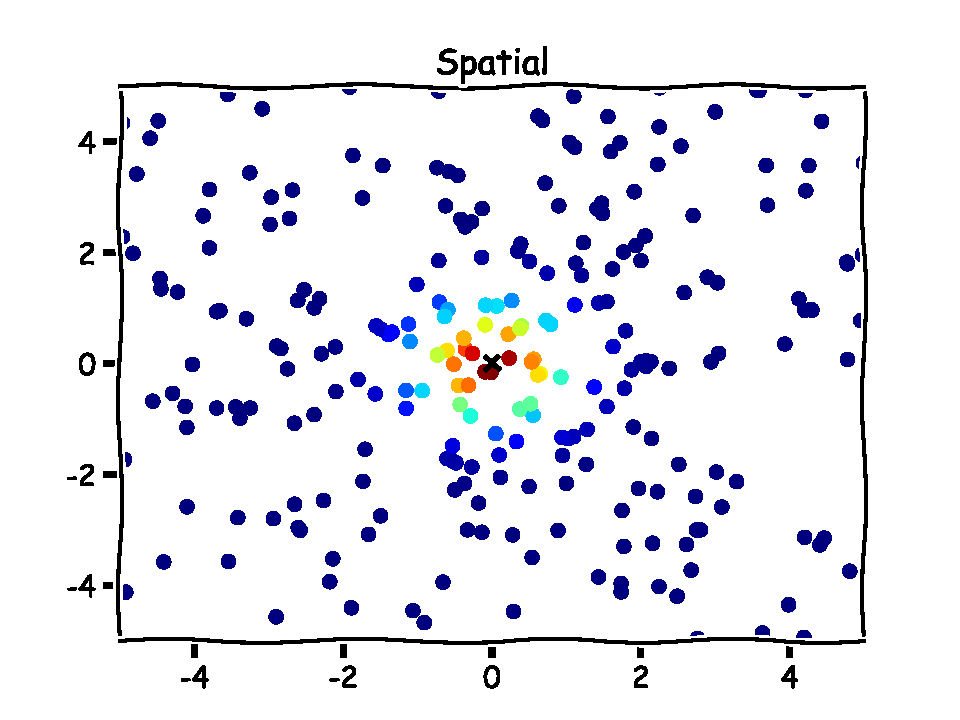
\includegraphics{llh/spatial}
	\caption{Visualisation of a spatial PDF.}
	\label{fig:spatial}
\end{marginfigure}

\begin{marginfigure}
	\centering \includegraphics{llh/energy}
	\caption{Visualisation of an energy proxy PDF.}
	\label{fig:energy}
\end{marginfigure}

Multiple box time PDFs are tested for a given source, and the one with the highest TS value is selected. Flares have both a start point, $T_{0}$, and end point, $T_{1}$, yielding two additional fit parameters. However, the likelihood landscape has discontinuities from when single neutrinos passing in/out boundary of the time PDF. Therefore, to avoid issues with minimisation by gradient descent, in  \flarestack{} the optimal flare is selected through a brute-force minimisation procedure. Though $T_{0}$ and $T_{1}$ are in principle continuous variables, the most significant possible cluster will always be one that begins and ends with the detection of a neutrino.

However, for N neutrinos in a dataset, there are $N \times (N-1)/2$ possible pairs to test. To further speed computation, a simplifying assumption is made that \emph{the most significant cluster will begin and end with signal-like neutrinos}. The $\mathcal{S}/\mathcal{B}$ ratio is calculated for all neutrinos, and only those with $\mathcal{S} > \mathcal{B}$ are considered sufficiently signal-like to test. This procedure is illustrated in Figure \ref{fig:time}.

\begin{marginfigure}
	\centering 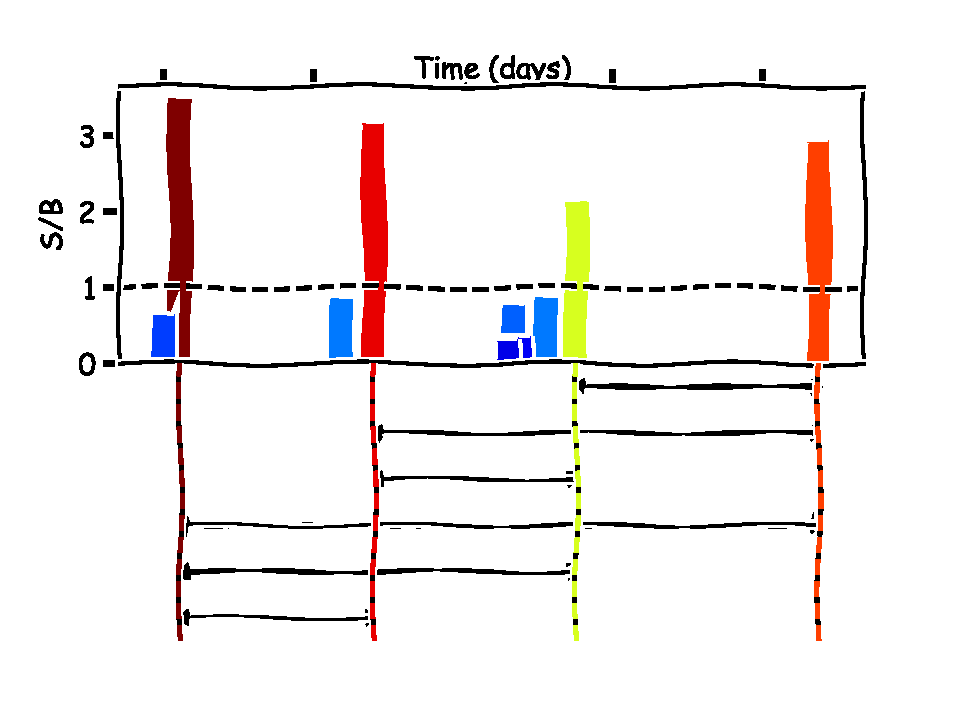
\includegraphics{llh/time}
	\caption{Visualisation of the cluster search algorithm.}
	\label{fig:time}
\end{marginfigure}

However, there is an inherent bias in such a cluster search, because there are many possible small clusters in a search window but very few possible large ones. Background fluctuations are preferentially found as small clusters. To counter this effect, a marginalisation term must be introduced to balance this bias, yielding a \emph{flare likelihood}. For a search window between $t_{0}$ and $t_{1}$, with a flare from $T_{0}$ to $T_{1}$, we find:

\begin{equation}
\Delta_{\textup{T, flare}} = \int_{T_{0}}^{T_{1}}f_{\textup{uptime}}(t) dt
\end{equation}

\begin{equation}
\Delta_{\textup{T, search}} = \int_{t_{0}}^{t_{1}}f_{\textup{uptime}}(t) dt
\end{equation}

\begin{equation}
\mathcal{L}(n_{s}, \gamma, T_{0}, T_{1}) = \prod_{i}^{N} \left(\frac{n_{s}}{N} \mathcal{S}(\theta_{i}, \gamma, T_{0}, T_{1}) + \frac{N - n_{s}}{N} \mathcal{B}(\theta_{i})  \right) \times \frac{\Delta_{\textup{T, flare}}}{\Delta_{\textup{T, search}}}
\end{equation}

An example of this cluster search, as used for the source AT2018cow (see Chapter \ref{ch:results}), demonstrates the impact on discovery potential. Given the additional degrees of freedom, there is more scope for background fluctuations, so the threshold for discovery is higher in the case that neutrino emission extends over the full search window. However, for shorter neutrino emission periods, the discovery potential is much reduced.

\begin{figure}[!ht]
	\centering 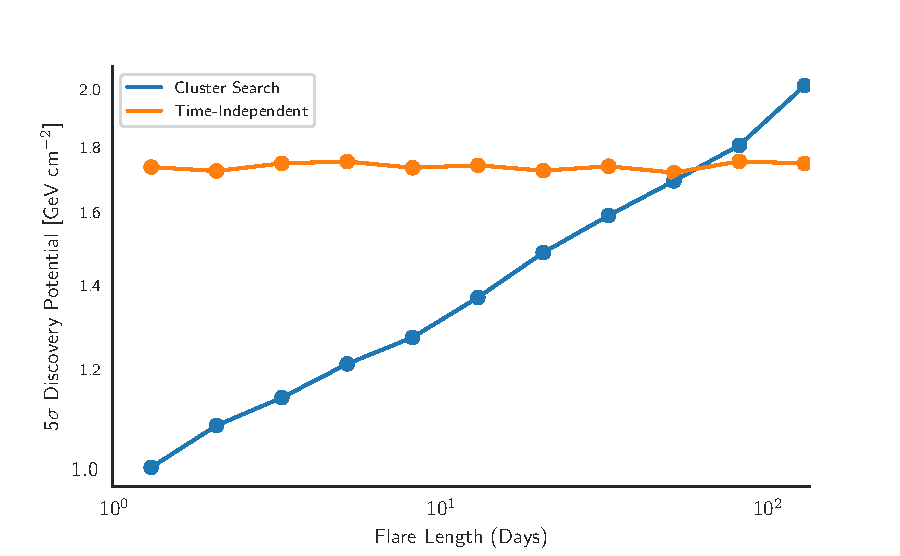
\includegraphics{llh/flare_vs_box}
	\caption{Estimated $5\sigma$ Discovery Potential for AT2018cow as a function of flare length, given in units of total fluence for an E$^{-2}$ spectrum over the 130 day search window.}
	\label{fig:DiscTime}
\end{figure}

\section{Fitting the relative source weights}
\label{sec:fit_weights}

The direct implementation of a well-defined $\mathcal{S}$ for a stacking analysis is the most powerful possible test, \emph{under the assumption that the relative distribution of the signal is known}. This condition can be satisfied when a specific model is tested that accurately predicts the relative number of signal events produced by each source in an ensemble. A prediction using multi-wavelength emission as a proxy, or expectations for a population of neutrino standard candles, are common assumptions. However, in an agnostic search for neutrino emission from a source ensemble, the uncertainty of our knowledge should be ideally implemented through priors on our expectations of neutrino emission from each source. The standard \emph{Point Source Likelihood} can be thought of as one extreme with maximum knowledge yielding $\delta$-function priors for the neutrino emission from each source. The other extreme is one of maximum ignorance, in which flat priors $n_{s, k}$ for each kth source is allowed to vary completely independently. In that case, we can replace the point-source likelihood (Equation \ref{eq:ps_llh}) with the \emph{multi-source likelihood}:

\begin{equation}
	\mathcal{L}(\vec{n_{s}}, \gamma) = \prod_{j}^{N} \left(\sum_{k} \left[ \frac{n_{s, k}}{N} \mathcal{S}_{k}(\theta_{j}, \gamma) \right]+ \frac{N - \sum_{k} \left[ n_{s, k} \right] }{N} \mathcal{B}(\theta_{j})  \right)
\end{equation}

This approach is commonly referred to as \emph{fitting the weights} of each source, in contrast to the standard method of \emph{fixed source weights}. Additional flexibility comes at the expense of more independent fit parameters, and thus a higher TS threshold to achieve fixed significance. In the limit of many sources, each with sub-unity neutrino expectations, the number of degrees of freedom would exceed the number of expected signal events. It is most useful for analysing a small number of sources, in which the relative neutrino distribution is not known, but for which multiple neutrinos would be expected. This likelihood is used for some results in this thesis (see Chapter \ref{ch:results}).

\section{Flarestack in practice}
The evaulation of this likelihood is time-consuming, and the implementation of this process in  \flarestack{} makes several standard simplifications to speed calculations \sidecite{stasik_thesis}. 


The first is the recognition that the parameters which maximise the likelihood will also maximise the likelihood ratio, and thus the test statistic. Rather than evaluating two independent likelihoods, we can instead directly evaluate the test statistic:

\begin{equation}
	TS = 2 \log \left( \frac{ \mathcal{L}(\hat{n}_{s}, \hat{\gamma}) }{\mathcal{L}(n_{s} = 0)} \right)
\end{equation}
\begin{equation}
TS = 2 \log  \frac{\prod_{j}^{N} \left(\frac{n_{s}}{N} \mathcal{S}(\theta_{j}, \gamma) + \frac{N - n_{s}}{N} \mathcal{B}(\theta_{j})  \right)}{\prod_{j}^{N}\mathcal{B}(\theta_{j})}
\end{equation}

By dividing this through, we find: 

\begin{equation}
	TS =  2 \log \left(  \prod_{j}^{N} \left(\frac{n_{s}}{N} \left[\frac{\mathcal{S}(\theta_{j}, \gamma)}{\mathcal{B}(\theta_{j})} \right] + 1 - \frac{n_{s}}{N} \right) \right) 
\end{equation}
\begin{equation}
	TS = 2 \sum_{j}^{N} \log \left(\frac{n_{s}}{N} \left[ \frac{\mathcal{S}(\theta_{j}, \gamma)}{\mathcal{B}(\theta_{j}) } - 1 \right] + 1 \right) 
\label{eq:TS_reduced}
\end{equation}

Equation \ref{eq:TS_reduced}  is faster to evaluate, because it bypasses the need to calculate both signal and background energy proxy PDFs explicitly. Instead, we can pre-computing the ratio $\frac{\mathcal{S}}{\mathcal{B}}$ for a variety of spectral indices, saving a per-event division calculation.

An additional simplifying assumption is that neutrinos are typically localised to a resolution of $\sim$1 degree, so events which lie many degrees from a source have a negligible probability of being signal. For events lying outside a \pm5 degree box, and those within a \pm5 degree box but with a spatial likelihood ratio less than $10^{-21}$, we make the approximation that $\mathcal{S} \approx 0$ so then $TS \approx 0$. Using the formulation in Equation \ref{eq:TS_reduced}, we see we can simply neglect to evaluate the likelihood for these events, without altering the final sum. This box cut thus removes the overwhelming majority of events from the likelihood evaluation step, yielding vast speed improvements while having a negligible impact on the fitting process.
